%% PNAStmpl.tex
%% Template file to use for PNAS articles prepared in LaTeX
%% Version: Apr 14, 2008


%%%%%%%%%%%%%%%%%%%%%%%%%%%%%%
%% BASIC CLASS FILE 
%% PNAStwo for two column articles is called by default.
%% Uncomment PNASone for single column articles. One column class
%% and style files are available upon request from pnas@nas.edu.
%% (uncomment means get rid of the '%' in front of the command)

%\documentclass{pnasone}
\documentclass{pnastwo}

%%%%%%%%%%%%%%%%%%%%%%%%%%%%%%
%% Changing position of text on physical page:
%% Since not all printers position
%% the printed page in the same place on the physical page,
%% you can change the position yourself here, if you need to:

% \advance\voffset -.5in % Minus dimension will raise the printed page on the 
                         %  physical page; positive dimension will lower it.

%% You may set the dimension to the size that you need.

%%%%%%%%%%%%%%%%%%%%%%%%%%%%%%
%% OPTIONAL GRAPHICS STYLE FILE

%% Requires graphics style file (graphicx.sty), used for inserting
%% .eps files into LaTeX articles.
%% Note that inclusion of .eps files is for your reference only;
%% when submitting to PNAS please submit figures separately.

%% Type into the square brackets the name of the driver program 
%% that you are using. If you don't know, try dvips, which is the
%% most common PC driver, or textures for the Mac. These are the options:

% [dvips], [xdvi], [dvipdf], [dvipdfm], [dvipdfmx], [pdftex], [dvipsone],
% [dviwindo], [emtex], [dviwin], [pctexps], [pctexwin], [pctexhp], [pctex32],
% [truetex], [tcidvi], [vtex], [oztex], [textures], [xetex]

%\usepackage[dvips]{graphicx}

%%%%%%%%%%%%%%%%%%%%%%%%%%%%%%
%% OPTIONAL POSTSCRIPT FONT FILES

%% PostScript font files: You may need to edit the PNASoneF.sty
%% or PNAStwoF.sty file to make the font names match those on your system. 
%% Alternatively, you can leave the font style file commands commented out
%% and typeset your article using the default Computer Modern 
%% fonts (recommended). If accepted, your article will be typeset
%% at PNAS using PostScript fonts.


% Choose PNASoneF for one column; PNAStwoF for two column:
%\usepackage{PNASoneF}
%\usepackage{PNAStwoF}

%%%%%%%%%%%%%%%%%%%%%%%%%%%%%%
%% ADDITIONAL OPTIONAL STYLE FILES

%% The AMS math files are commonly used to gain access to useful features
%% like extended math fonts and math commands.

\usepackage{amssymb,amsfonts,amsmath,amsthm}

%%%%%%%%%%%%%%%%%%%%%%%%%%%%%%
%% OPTIONAL MACRO FILES
%% Insert self-defined macros here.
%% \newcommand definitions are recommended; \def definitions are supported

%\newcommand{\mfrac}[2]{\frac{\displaystyle #1}{\displaystyle #2}}
%\def\s{\sigma}

%auto-ignore
%!TEX root = pnas.tex

\def\bc{{\mathcal B}}
\def\btc{{\mathcal{BT}}}

\newcommand{\HC}{\operatorname{Hoch}}
\newcommand{\HH}{\operatorname{HH}}

\newcommand{\CM}[2]{C_*(\Maps(#1 \to #2))}
\newcommand{\CD}[1]{C_*(\Diff(#1))}
\newcommand{\CH}[1]{CH_*(#1)}

\newcommand{\cl}[1]{\underrightarrow{#1}}

\newcommand{\Set}{\text{\textbf{Set}}}
\newcommand{\Vect}{\text{\textbf{Vect}}}
\newcommand{\Kom}{\text{\textbf{Kom}}}
\newcommand{\Cat}{\mathcal{C}}

\newcommand{\cell}{\mathfrak{D}}

\newcommand{\into}{\hookrightarrow}
\newcommand{\onto}{\twoheadrightarrow}
\newcommand{\iso}{\cong}
\newcommand{\quism}{\underset{\text{q.i.}}{\simeq}}
\newcommand{\htpy}{\simeq}
\newcommand{\actsOn}{\circlearrowright}
\newcommand{\xto}[1]{\xrightarrow{#1}}
\newcommand{\isoto}{\xto{\iso}}
\newcommand{\quismto}{\xrightarrow[\text{q.i.}]{\iso}}
\newcommand{\diffeoto}{\xrightarrow[\text{diffeo}]{\iso}}
\newcommand{\htpyto}{\xrightarrow[\text{htpy}]{\htpy}}

\newcommand{\directSum}{\oplus}
\newcommand{\DirectSum}{\bigoplus}
\newcommand{\tensor}{\otimes}
\newcommand{\Tensor}{\bigotimes}

\newcommand{\selfarrow}{\ensuremath{\smash{\tikz[baseline]{\clip (0,0.36) rectangle (0.48,-0.16); \draw[->] (0,0.2) .. controls (0.6,0.8) and (0.6,-0.6) .. (0,0);}}}}

\newcommand{\bdy}{\partial}
\newcommand{\compose}{\circ}
\newcommand{\eset}{\emptyset}

\newcommand{\id}{\boldsymbol{1}}

\newtheorem{property}{Property}
\newtheorem{prop}{Proposition}
\newtheorem{thm}[prop]{Theorem}

\newenvironment{rem}{\noindent\textsl{Remark.}}{}

% \mathrlap -- a horizontal \smash--------------------------------
% For comparison, the existing overlap macros:
% \def\llap#1{\hbox to 0pt{\hss#1}}
% \def\rlap#1{\hbox to 0pt{#1\hss}}
\def\clap#1{\hbox to 0pt{\hss#1\hss}}
\def\mathllap{\mathpalette\mathllapinternal}
\def\mathrlap{\mathpalette\mathrlapinternal}
\def\mathclap{\mathpalette\mathclapinternal}
\def\mathllapinternal#1#2{%
\llap{$\mathsurround=0pt#1{#2}$}}
\def\mathrlapinternal#1#2{%
\rlap{$\mathsurround=0pt#1{#2}$}}
\def\mathclapinternal#1#2{%
\clap{$\mathsurround=0pt#1{#2}$}}

% references

\newcommand{\arxiv}[1]{\href{http://arxiv.org/abs/#1}{\tt arXiv:\nolinkurl{#1}}}
\newcommand{\doi}[1]{\href{http://dx.doi.org/#1}{{\tt DOI:#1}}}
\newcommand{\euclid}[1]{\href{http://projecteuclid.org/euclid.cmp/#1}{{\tt at Project Euclid: #1}}}
\newcommand{\mathscinet}[1]{\href{http://www.ams.org/mathscinet-getitem?mr=#1}{\tt #1}}
\newcommand{\googlebooks}[1]{(preview at \href{http://books.google.com/books?id=#1}{google books})}



% packages

\usepackage{tikz}
\usetikzlibrary{shapes}
\usetikzlibrary{backgrounds}
\usetikzlibrary{decorations,decorations.pathreplacing}
\usetikzlibrary{fit,calc,through}

\usepackage[all,color]{xy}
\SelectTips{cm}{}

\usepackage[pdftex,plainpages=false,hypertexnames=false,pdfpagelabels]{hyperref}

\usepackage{xcolor}
\definecolor{dark-red}{rgb}{0.7,0.25,0.25}
\definecolor{dark-blue}{rgb}{0.15,0.15,0.55}
\definecolor{medium-blue}{rgb}{0,0,0.65}

\hypersetup{
    colorlinks, linkcolor={dark-red},
    citecolor={dark-blue}, urlcolor={medium-blue}
}


%!TEX root = ../blob1.tex

%%%%% excerpts from KW's include file of standard macros

\def\z{\mathbb{Z}}
\def\r{\mathbb{R}}
\def\c{\mathbb{C}}
\def\t{\mathbb{T}}

\def\du{\sqcup}
\def\bd{\partial}
\def\sub{\subset}
\def\subeq{\subseteq}
\def\sup{\supset}
%\def\setmin{\smallsetminus}
\def\setmin{\setminus}
\def\ep{\epsilon}
\def\sgl{_\mathrm{gl}}
\def\op{^\mathrm{op}}
\def\deq{\stackrel{\mathrm{def}}{=}}
\def\pd#1#2{\frac{\partial #1}{\partial #2}}
\def\lf{\overline{\cC}}
\def\ot{\otimes}

\def\nn#1{{{\it \small [#1]}}}
\long\def\noop#1{}

% equations
\newcommand{\eq}[1]{\begin{displaymath}#1\end{displaymath}}
\newcommand{\eqar}[1]{\begin{eqnarray*}#1\end{eqnarray*}}
\newcommand{\eqspl}[1]{\begin{displaymath}\begin{split}#1\end{split}\end{displaymath}}

% tricky way to iterate macros over a list
\def\semicolon{;}
\def\applytolist#1{
    \expandafter\def\csname multi#1\endcsname##1{
        \def\multiack{##1}\ifx\multiack\semicolon
            \def\next{\relax}
        \else
            \csname #1\endcsname{##1}
            \def\next{\csname multi#1\endcsname}
        \fi
        \next}
    \csname multi#1\endcsname}

% \def\cA{{\cal A}} for A..Z
\def\calc#1{\expandafter\def\csname c#1\endcsname{{\mathcal #1}}}
\applytolist{calc}QWERTYUIOPLKJHGFDSAZXCVBNM;

% \DeclareMathOperator{\pr}{pr} etc.
\def\declaremathop#1{\expandafter\DeclareMathOperator\csname #1\endcsname{#1}}
\applytolist{declaremathop}{pr}{im}{gl}{ev}{coinv}{tr}{rot}{Eq}{obj}{mor}{ob}{Rep}{Tet}{cat}{Maps}{Diff}{Homeo}{sign}{supp}{Nbd};



%%%%%% end excerpt




%%%%%%%%%%%%%%%%%%%%%%%%%%%%%%
%% Don't type in anything in the following section:
%%%%%%%%%%%%
%% For PNAS Only:
\contributor{Submitted to Proceedings
of the National Academy of Sciences of the United States of America}
%\url{www.pnas.org/cgi/doi/10.1073/pnas.0709640104}
\copyrightyear{2008}
\issuedate{Issue Date}
\volume{Volume}
\issuenumber{Issue Number}
%%%%%%%%%%%%

\begin{document}

%%%%%%%%%%%%%%%%%%%%%%%%%%%%%%


%% For titles, only capitalize the first letter
%% \title{Almost sharp fronts for the surface quasi-geostrophic equation}

\title{The blob complex}


%% Enter authors via the \author command.  
%% Use \affil to define affiliations.
%% (Leave no spaces between author name and \affil command)

%% Note that the \thanks{} command has been disabled in favor of
%% a generic, reserved space for PNAS publication footnotes.

%% \author{<author name>
%% \affil{<number>}{<Institution>}} One number for each institution.
%% The same number should be used for authors that
%% are affiliated with the same institution, after the first time
%% only the number is needed, ie, \affil{number}{text}, \affil{number}{}
%% Then, before last author ...
%% \and
%% \author{<author name>
%% \affil{<number>}{}}

%% For example, assuming Garcia and Sonnery are both affiliated with
%% Universidad de Murcia:
%% \author{Roberta Graff\affil{1}{University of Cambridge, Cambridge,
%% United Kingdom},
%% Javier de Ruiz Garcia\affil{2}{Universidad de Murcia, Bioquimica y Biologia
%% Molecular, Murcia, Spain}, \and Franklin Sonnery\affil{2}{}}

\author{Scott Morrison\affil{1}{Miller Institute for Basic Research, UC Berkeley, CA 94704, USA} \and Kevin Walker\affil{2}{Microsoft Station Q, 2243 CNSI Building, UC Santa Barbara, CA 93106, USA}}

\contributor{Submitted to Proceedings of the National Academy of Sciences
of the United States of America}

%% The \maketitle command is necessary to build the title page.
\maketitle

%%%%%%%%%%%%%%%%%%%%%%%%%%%%%%%%%%%%%%%%%%%%%%%%%%%%%%%%%%%%%%%%
\begin{article}

\begin{abstract} -- enter abstract text here -- \end{abstract}


%% When adding keywords, separate each term with a straight line: |
\keywords{n-categories | topological quantum field theory | hochschild homology}

%% Optional for entering abbreviations, separate the abbreviation from
%% its definition with a comma, separate each pair with a semicolon:
%% for example:
%% \abbreviations{SAM, self-assembled monolayer; OTS,
%% octadecyltrichlorosilane}

% \abbreviations{}

%% The first letter of the article should be drop cap: \dropcap{}
%\dropcap{I}n this article we study the evolution of ''almost-sharp'' fronts

%% Enter the text of your article beginning here and ending before
%% \begin{acknowledgements}
%% Section head commands for your reference:
%% \section{}
%% \subsection{}
%% \subsubsection{}

\nn{
background: TQFTs are important, historically, semisimple categories well-understood.
Many new examples arising recently which do not fit this framework, e.g. SW and OS theory.
These have more complicated gluing formulas (\cite{1003.0598,1005.1248}, etc); 
it would be nice to give generalized TQFT axioms that encompass these.
Triangulated categories are important; often calculations are via exact sequences,
and the standard TQFT constructions are quotients, which destroy exactness.
A first attempt to deal with this might be to replace all the tensor products in gluing formulas
with derived tensor products (cite Kh?).
However, in this approach it's probably difficult to prove invariance of constructions,
because they depend on explicit presentations of the manifold.
We'll give a manifestly invariant construction,
and deduce gluing formulas based on derived (actually, $A_\infty$) tensor products.}

\section{Definitions}
\subsection{$n$-categories} \mbox{}

\nn{rough draft of n-cat stuff...}

\nn{maybe say something about goals: well-suited to TQFTs; avoid proliferation of coherency axioms;
non-recursive (n-cats not defined n terms of (n-1)-cats; easy to show that the motivating
examples satisfy the axioms; strong duality; both plain and infty case;
(?) easy to see that axioms are correct, in the sense of nothing missing (need
to say this better if we keep it)}

\nn{maybe: the typical n-cat definition tries to do two things at once: (1) give a list of basic properties
which are weak enough to include the basic examples and strong enough to support the proofs
of the main theorems; and (2) specify a minimal set of generators and/or axioms.
We separate these two tasks, and address only the first, which becomes much easier when not burdened by the second.
More specifically, life is easier when working with maximal, rather than minimal, collections of axioms.}

\nn{say something about defining plain and infty cases simultaneously}

There are five basic ingredients of an $n$-category definition:
$k$-morphisms (for $0\le k \le n$), domain and range, composition,
identity morphisms, and special behavior in dimension $n$ (e.g. enrichment
in some auxiliary category, or strict associativity instead of weak associativity).
We will treat each of these in turn.

To motivate our morphism axiom, consider the venerable notion of the Moore loop space
\cite[\S 2.2]{MR505692}.
In the standard definition of a loop space, loops are always parameterized by the unit interval $I = [0,1]$,
so composition of loops requires a reparameterization $I\cup I \cong I$, and this leads to a proliferation
of higher associativity relations.
While this proliferation is manageable for 1-categories (and indeed leads to an elegant theory
of Stasheff polyhedra and $A_\infty$ categories), it becomes undesirably complex for higher categories.
In a Moore loop space, we have a separate space $\Omega_r$ for each interval $[0,r]$, and a 
{\it strictly associative} composition $\Omega_r\times \Omega_s\to \Omega_{r+s}$.
Thus we can have the simplicity of strict associativity in exchange for more morphisms.
We wish to imitate this strategy in higher categories.
Because we are mainly interested in the case of strong duality, we replace the intervals $[0,r]$ not with
a product of $k$ intervals \nn{cf xxxx} but rather with any $k$-ball, that is, any $k$-manifold which is homeomorphic
to the standard $k$-ball $B^k$.
\nn{maybe add that in addition we want functoriality}

We haven't said precisely what sort of balls we are considering,
because we prefer to let this detail be a parameter in the definition.
It is useful to consider unoriented, oriented, Spin and $\mbox{Pin}_\pm$ balls.
Also useful are more exotic structures, such as balls equipped with a map to some target space,
or equipped with $m$ independent vector fields.
(The latter structure would model $n$-categories with less duality than we usually assume.)

%In fact, the axioms here may easily be varied by considering balls with structure (e.g. $m$ independent vector fields, a map to some target space, etc.). Such variations are useful for axiomatizing categories with less duality, and also as technical tools in proofs.

\begin{axiom}[Morphisms]
\label{axiom:morphisms}
For each $0 \le k \le n$, we have a functor $\cC_k$ from 
the category of $k$-balls and 
homeomorphisms to the category of sets and bijections.
\end{axiom}

Note that the functoriality in the above axiom allows us to operate via
homeomorphisms which are not the identity on the boundary of the $k$-ball.
The action of these homeomorphisms gives the ``strong duality" structure.
As such, we don't subdivide the boundary of a morphism
into domain and range --- the duality operations can convert between domain and range.

Later \todo{} we inductively define an extension of the functors $\cC_k$ to functors $\cl{\cC}_k$ from arbitrary manifolds to sets. We need the restriction of these functors to $k$-spheres, for $k<n$, for the next axiom.

\begin{axiom}[Boundaries]\label{nca-boundary}
For each $k$-ball $X$, we have a map of sets $\bd: \cC_k(X)\to \cl{\cC}_{k-1}(\bd X)$.
These maps, for various $X$, comprise a natural transformation of functors.
\end{axiom}

For $c\in \cl{\cC}_{k-1}(\bd X)$ we define $\cC_k(X; c) = \bd^{-1}(c)$.

Many of the examples we are interested in are enriched in some auxiliary category $\cS$
(e.g. vector spaces or rings, or, in the $A_\infty$ case, chain complexes or topological spaces).
This means that in the top dimension $k=n$ the sets $\cC_n(X; c)$ have the structure
of an object of $\cS$, and all of the structure maps of the category (above and below) are
compatible with the $\cS$ structure on $\cC_n(X; c)$.


Given two hemispheres (a `domain' and `range') that agree on the equator, we need to be able to assemble them into a boundary value of the entire sphere.

\begin{lem}
\label{lem:domain-and-range}
Let $S = B_1 \cup_E B_2$, where $S$ is a $k{-}1$-sphere $(1\le k\le n)$,
$B_i$ is a $k{-}1$-ball, and $E = B_1\cap B_2$ is a $k{-}2$-sphere (Figure \ref{blah3}).
Let $\cC(B_1) \times_{\cl{\cC}(E)} \cC(B_2)$ denote the fibered product of the 
two maps $\bd: \cC(B_i)\to \cl{\cC}(E)$.
Then we have an injective map
\[
	\gl_E : \cC(B_1) \times_{\cl{\cC}(E)} \cC(B_2) \into \cl{\cC}(S)
\]
which is natural with respect to the actions of homeomorphisms.
%(When $k=1$ we stipulate that $\cl{\cC}(E)$ is a point, so that the above fibered product
%becomes a normal product.)
\end{lem}

If $\bdy B = S$, we denote $\bdy^{-1}(\im(\gl_E))$ by $\cC(B)_E$.

\begin{axiom}[Gluing]
\label{axiom:composition}
Let $B = B_1 \cup_Y B_2$, where $B$, $B_1$ and $B_2$ are $k$-balls ($0\le k\le n$)
and $Y = B_1\cap B_2$ is a $k{-}1$-ball (Figure \ref{blah5}).
Let $E = \bd Y$, which is a $k{-}2$-sphere.
%Note that each of $B$, $B_1$ and $B_2$ has its boundary split into two $k{-}1$-balls by $E$.
We have restriction maps $\cC(B_i)_E \to \cC(Y)$.
Let $\cC(B_1)_E \times_{\cC(Y)} \cC(B_2)_E$ denote the fibered product of these two maps. 
We have a map
\[
	\gl_Y : \cC(B_1)_E \times_{\cC(Y)} \cC(B_2)_E \to \cC(B)_E
\]
which is natural with respect to the actions of homeomorphisms, and also compatible with restrictions
to the intersection of the boundaries of $B$ and $B_i$.
If $k < n$,
or if $k=n$ and we are in the $A_\infty$ case, 
we require that $\gl_Y$ is injective.
(For $k=n$ in the plain (non-$A_\infty$) case, see below.)
\end{axiom}

\begin{axiom}[Strict associativity] \label{nca-assoc}
The gluing maps above are strictly associative.
Given any decomposition of a ball $B$ into smaller balls
$$\bigsqcup B_i \to B,$$ 
any sequence of gluings (where all the intermediate steps are also disjoint unions of balls) yields the same result.
\end{axiom}
For the next axiom, a \emph{pinched product} is a map locally modeled on a degeneracy map between simplices.
\begin{axiom}[Product (identity) morphisms]
\label{axiom:product}
For each pinched product $\pi:E\to X$, with $X$ a $k$-ball and $E$ a $k{+}m$-ball ($m\ge 1$),
there is a map $\pi^*:\cC(X)\to \cC(E)$.
These maps must be
\begin{enumerate}
\item natural with respect to maps of pinched products,
\item functorial with respect to composition of pinched products, 
\item compatible with gluing and restriction of pinched products.
\end{enumerate}

%%% begin noop %%%
% this was the original list of conditions, which I've replaced with the much terser list above -S
\noop{
These maps must satisfy the following conditions.
\begin{enumerate}
\item
If $\pi:E\to X$ and $\pi':E'\to X'$ are pinched products, and
if $f:X\to X'$ and $\tilde{f}:E \to E'$ are maps such that the diagram
\[ \xymatrix{
	E \ar[r]^{\tilde{f}} \ar[d]_{\pi} & E' \ar[d]^{\pi'} \\
	X \ar[r]^{f} & X'
} \]
commutes, then we have 
\[
	\pi'^*\circ f = \tilde{f}\circ \pi^*.
\]
\item
Product morphisms are compatible with gluing.
Let $\pi:E\to X$, $\pi_1:E_1\to X_1$, and $\pi_2:E_2\to X_2$ 
be pinched products with $E = E_1\cup E_2$.
Let $a\in \cC(X)$, and let $a_i$ denote the restriction of $a$ to $X_i\sub X$.
Then 
\[
	\pi^*(a) = \pi_1^*(a_1)\bullet \pi_2^*(a_2) .
\]
\item
Product morphisms are associative.
If $\pi:E\to X$ and $\rho:D\to E$ are pinched products then
\[
	\rho^*\circ\pi^* = (\pi\circ\rho)^* .
\]
\item
Product morphisms are compatible with restriction.
If we have a commutative diagram
\[ \xymatrix{
	D \ar@{^(->}[r] \ar[d]_{\rho} & E \ar[d]^{\pi} \\
	Y \ar@{^(->}[r] & X
} \]
such that $\rho$ and $\pi$ are pinched products, then
\[
	\res_D\circ\pi^* = \rho^*\circ\res_Y .
\]
\end{enumerate}
} %%% end \noop %%%
\end{axiom}
\begin{axiom}[\textup{\textbf{[plain  version]}} Extended isotopy invariance in dimension $n$.]
\label{axiom:extended-isotopies}
Let $X$ be an $n$-ball and $f: X\to X$ be a homeomorphism which restricts
to the identity on $\bd X$ and isotopic (rel boundary) to the identity.
Then $f$ acts trivially on $\cC(X)$.
In addition, collar maps act trivially on $\cC(X)$.
\end{axiom}

\nn{need to define collar maps}

\smallskip

For $A_\infty$ $n$-categories, we replace
isotopy invariance with the requirement that families of homeomorphisms act.
For the moment, assume that our $n$-morphisms are enriched over chain complexes.
Let $\Homeo_\bd(X)$ denote homeomorphisms of $X$ which fix $\bd X$ and
$C_*(\Homeo_\bd(X))$ denote the singular chains on this space.


\begin{axiom}[\textup{\textbf{[$A_\infty$ version]}} Families of homeomorphisms act in dimension $n$.]
\label{axiom:families}
For each $n$-ball $X$ and each $c\in \cl{\cC}(\bd X)$ we have a map of chain complexes
\[
	C_*(\Homeo_\bd(X))\ot \cC(X; c) \to \cC(X; c) .
\]
These action maps are required to be associative up to homotopy,
and also compatible with composition (gluing) in the sense that
a diagram like the one in Theorem \ref{thm:CH} commutes.
\end{axiom}


\todo{
Decide if we need a friendlier, skein-module version.
}

\subsection{Example (the fundamental $n$-groupoid)}
We will define $\pi_{\le n}(T)$, the fundamental $n$-groupoid of a topological space $T$.
When $X$ is a $k$-ball with $k<n$, define $\pi_{\le n}(T)(X)$
to be the set of continuous maps from $X$ to $T$.
When $X$ is an $n$-ball, define $\pi_{\le n}(T)(X)$ to be homotopy classes (rel boundary) of such maps.
Define boundary restrictions and gluing in the obvious way.
If $\rho:E\to X$ is a pinched product and $f:X\to T$ is a $k$-morphism,
define the product morphism $\rho^*(f)$ to be $f\circ\rho$.

We can also define an $A_\infty$ version $\pi_{\le n}^\infty(T)$ of the fundamental $n$-groupoid.
For $X$ an $n$-ball define $\pi_{\le n}^\infty(T)(X)$ to be the space of all maps from $X$ to $T$
(if we are enriching over spaces) or the singular chains on that space (if we are enriching over chain complexes).


\subsection{Example (string diagrams)}
Fix a `traditional' $n$-category $C$ with strong duality (e.g.\ a pivotal 2-category).
Let $X$ be a $k$-ball and define $\cS_C(X)$ to be the set of $C$ string diagrams drawn on $X$;
that is, certain cell complexes embedded in $X$, with the codimension-$j$ cells labeled by $j$-morphisms of $C$.
If $X$ is an $n$-ball, identify two such string diagrams if they evaluate to the same $n$-morphism of $C$.
Boundary restrictions and gluing are again straightforward to define.
Define product morphisms via product cell decompositions.


\nn{also do bordism category?}

\subsection{The blob complex}
\subsubsection{Decompositions of manifolds}

\nn{KW: I'm inclined to suppress all discussion of the subtleties of decompositions.
Maybe just a single remark that we are omitting some details which appear in our
longer paper.}
\nn{SM: for now I disagree: the space expense is pretty minor, and it allows us to be ``in principle" complete. Let's see how we go for length.}
\nn{KW: It's not the length I'm worried about --- I was worried about distracting the reader
with an arcane technical issue.  But we can decide later.}

A \emph{ball decomposition} of $W$ is a 
sequence of gluings $M_0\to M_1\to\cdots\to M_m = W$ such that $M_0$ is a disjoint union of balls
$\du_a X_a$ and each $M_i$ is a manifold.
If $X_a$ is some component of $M_0$, its image in $W$ need not be a ball; $\bd X_a$ may have been glued to itself.
A {\it permissible decomposition} of $W$ is a map
\[
	\coprod_a X_a \to W,
\]
which can be completed to a ball decomposition $\du_a X_a = M_0\to\cdots\to M_m = W$.
A permissible decomposition is weaker than a ball decomposition; we forget the order in which the balls
are glued up to yield $W$, and just require that there is some non-pathological way to do this.

Given permissible decompositions $x = \{X_a\}$ and $y = \{Y_b\}$ of $W$, we say that $x$ is a refinement
of $y$, or write $x \le y$, if there is a ball decomposition $\du_a X_a = M_0\to\cdots\to M_m = W$
with $\du_b Y_b = M_i$ for some $i$.

\begin{defn}
The poset $\cell(W)$ has objects the permissible decompositions of $W$, 
and a unique morphism from $x$ to $y$ if and only if $x$ is a refinement of $y$.
See Figure \ref{partofJfig} for an example.
\end{defn}

This poset in fact has more structure, since we can glue together permissible decompositions of $W_1$ and $W_2$ to obtain a permissible decomposition of $W_1 \sqcup W_2$. 

An $n$-category $\cC$ determines 
a functor $\psi_{\cC;W}$ from $\cell(W)$ to the category of sets 
(possibly with additional structure if $k=n$).
Each $k$-ball $X$ of a decomposition $y$ of $W$ has its boundary decomposed into $k{-}1$-balls,
and there is a subset $\cC(X)\spl \sub \cC(X)$ of morphisms whose boundaries
are splittable along this decomposition.

\begin{defn}
Define the functor $\psi_{\cC;W} : \cell(W) \to \Set$ as follows.
For a decomposition $x = \bigsqcup_a X_a$ in $\cell(W)$, $\psi_{\cC;W}(x)$ is the subset
\begin{equation*}
%\label{eq:psi-C}
	\psi_{\cC;W}(x) \sub \prod_a \cC(X_a)\spl
\end{equation*}
where the restrictions to the various pieces of shared boundaries amongst the cells
$X_a$ all agree (this is a fibered product of all the labels of $n$-cells over the labels of $n-1$-cells). When $k=n$, the `subset' and `product' in the above formula should be interpreted in the appropriate enriching category.
If $x$ is a refinement of $y$, the map $\psi_{\cC;W}(x) \to \psi_{\cC;W}(y)$ is given by the composition maps of $\cC$.
\end{defn}

We will use the term `field on $W$' to refer to \nn{a point} of this functor,
that is, a permissible decomposition $x$ of $W$ together with an element of $\psi_{\cC;W}(x)$.

\todo{Mention that the axioms for $n$-categories can be stated in terms of decompositions of balls?}

\subsubsection{Homotopy colimits}
\nn{Motivation: How can we extend an $n$-category from balls to arbitrary manifolds?}

We can now give a straightforward but rather abstract definition of the blob complex of an $n$-manifold $W$
with coefficients in the $n$-category $\cC$ as the homotopy colimit along $\cell(W)$
of the functor $\psi_{\cC; W}$ described above. We write this as $\clh{\cC}(W)$.

An explicit realization of the homotopy colimit is provided by the simplices of the functor $\psi_{\cC; W}$. That is, $$\clh{\cC}(W) = \DirectSum_{\bar{x}} \psi_{\cC; W}(x_0)[m],$$ where $\bar{x} = x_0 \leq \cdots \leq x_m$ is a simplex in $\cell(W)$. The differential acts on $(\bar{x},a)$ (here $a \in \psi_{\cC; W}(x_0)$) as
$$\bdy (\bar{x},a) = (\bar{x}, \bdy a) + (-1)^{\deg a} \left( (d_0 \bar{x}, g(a)) + \sum_{i=1}^m (-1)^i (d_i \bar{x}, a) \right)$$
where $g$ is the gluing map from $x_0$ to $x_1$, and $d_i \bar{x}$ denotes the $i$-th face of the simplex $\bar{x}$.

Alternatively, we can take advantage of the product structure on $\cell(W)$ to realize the homotopy colimit via the cone-product polyhedra in $\cell(W)$. A cone-product polyhedra is obtained from a point by successively taking the cone or taking the product with another cone-product polyhedron. Just as simplices correspond to linear graphs, cone-product polyheda correspond to directed trees: taking cone adds a new root before the existing root, and taking product identifies the roots of several trees. The `local homotopy colimit' is then defined according to the same formula as above, but with $x$ a cone-product polyhedron in $\cell(W)$.
A Eilenberg-Zilber subdivision argument shows this is the same as the usual realization.

When $\cC$ is a topological $n$-category,
the flexibility available in the construction of a homotopy colimit allows
us to give a much more explicit description of the blob complex which we'll write as $\bc_*(W; \cC)$.

We say a collection of balls $\{B_i\}$ in a manifold $W$ is \emph{permissible}
if there exists a permissible decomposition $M_0\to\cdots\to M_m = W$ such that
each $B_i$ appears as a connected component of one of the $M_j$. Note that this allows the balls to be pairwise either disjoint or nested. Such a collection of balls cuts $W$ into pieces, the connected components of $W \setminus \bigcup \bdy B_i$. These pieces need not be manifolds, but they do automatically have permissible decompositions.

The $k$-blob group $\bc_k(W; \cC)$ is generated by the $k$-blob diagrams. A $k$-blob diagram consists of
\begin{itemize}
\item a permissible collection of $k$ embedded balls,
\item an ordering of the balls, and
\item for each resulting piece of $W$, a field,
\end{itemize}
such that for any innermost blob $B$, the field on $B$ goes to zero under the gluing map from $\cC$. We call such a field a `null field on $B$'.

The differential acts on a $k$-blob diagram by summing over ways to forget one of the $k$ blobs, with signs given by the ordering.

We now spell this out for some small values of $k$. For $k=0$, the $0$-blob group is simply fields on $W$. For $k=1$, a generator consists of a field on $W$ and a ball, such that the restriction of the field to that ball is a null field. The differential simply forgets the ball. Thus we see that $H_0$ of the blob complex is the quotient of fields by fields which are null on some ball.

For $k=2$, we have a two types of generators; they each consists of a field $f$ on $W$, and two balls $B_1$ and $B_2$. In the first case, the balls are disjoint, and $f$ restricted to either of the $B_i$ is a null field. In the second case, the balls are properly nested, say $B_1 \subset B_2$, and $f$ restricted to $B_1$ is null. Note that this implies that $f$ restricted to $B_2$ is also null, by the associativity of the gluing operation. This ensures that the differential is well-defined.

\section{Properties of the blob complex}
\subsection{Formal properties}
\label{sec:properties}
The blob complex enjoys the following list of formal properties. The first three properties are immediate from the definitions.

\begin{property}[Functoriality]
\label{property:functoriality}%
The blob complex is functorial with respect to homeomorphisms.
That is, 
for a fixed $n$-category $\cC$, the association
\begin{equation*}
X \mapsto \bc_*(X; \cC)
\end{equation*}
is a functor from $n$-manifolds and homeomorphisms between them to chain 
complexes and isomorphisms between them.
\end{property}
As a consequence, there is an action of $\Homeo(X)$ on the chain complex $\bc_*(X; \cC)$; 
this action is extended to all of $C_*(\Homeo(X))$ in Theorem \ref{thm:CH} below.

\begin{property}[Disjoint union]
\label{property:disjoint-union}
The blob complex of a disjoint union is naturally isomorphic to the tensor product of the blob complexes.
\begin{equation*}
\bc_*(X_1 \du X_2) \iso \bc_*(X_1) \tensor \bc_*(X_2)
\end{equation*}
\end{property}

If an $n$-manifold $X$ contains $Y \sqcup Y^\text{op}$ (we allow $Y = \eset$) as a codimension $0$ submanifold of its boundary, 
write $X \bigcup_{Y}\selfarrow$ for the manifold obtained by gluing together $Y$ and $Y^\text{op}$.
\begin{property}[Gluing map]
\label{property:gluing-map}%
%If $X_1$ and $X_2$ are $n$-manifolds, with $Y$ a codimension $0$-submanifold of $\bdy X_1$, and $Y^{\text{op}}$ a codimension $0$-submanifold of $\bdy X_2$, there is a chain map
%\begin{equation*}
%\gl_Y: \bc_*(X_1) \tensor \bc_*(X_2) \to \bc_*(X_1 \cup_Y X_2).
%\end{equation*}
Given a gluing $X \to X_\mathrm{gl}$, there is
a map
\[
	\bc_*(X) \to \bc_*(X \bigcup_{Y}\selfarrow),
\]
natural with respect to homeomorphisms, and associative with respect to iterated gluings.
\end{property}

\begin{property}[Contractibility]
\label{property:contractibility}%
The blob complex on an $n$-ball is contractible in the sense 
that it is homotopic to its $0$-th homology, and this is just the vector space associated to the ball by the $n$-category.
\begin{equation*}
\xymatrix{\bc_*(B^n;\cC) \ar[r]^(0.4){\iso}_(0.4){\text{qi}} & H_0(\bc_*(B^n;\cC)) \ar[r]^(0.6)\iso & \cC(B^n)}
\end{equation*}
\end{property}
\nn{maybe should say something about the $A_\infty$ case}

\begin{proof}(Sketch)
For $k\ge 1$, the contracting homotopy sends a $k$-blob diagram to the $(k{+}1)$-blob diagram
obtained by adding an outer $(k{+}1)$-st blob consisting of all $B^n$.
For $k=0$ we choose a splitting $s: H_0(\bc_*(B^n)) \to \bc_0(B^n)$ and send 
$x\in \bc_0(B^n)$ to $x - s([x])$, where $[x]$ denotes the image of $x$ in $H_0(\bc_*(B^n))$.
\end{proof}

\subsection{Specializations}
\label{sec:specializations}

The blob complex has two important special cases.

\begin{thm}[Skein modules]
\label{thm:skein-modules}
\nn{Plain n-categories only?}
The $0$-th blob homology of $X$ is the usual 
(dual) TQFT Hilbert space (a.k.a.\ skein module) associated to $X$
by $\cC$.
\begin{equation*}
H_0(\bc_*(X;\cC)) \iso A_{\cC}(X)
\end{equation*}
\end{thm}
This follows from the fact that the $0$-th homology of a homotopy colimit is the usual colimit, or directly from the explicit description of the blob complex.

\begin{thm}[Hochschild homology when $X=S^1$]
\label{thm:hochschild}
The blob complex for a $1$-category $\cC$ on the circle is
quasi-isomorphic to the Hochschild complex.
\begin{equation*}
\xymatrix{\bc_*(S^1;\cC) \ar[r]^(0.47){\iso}_(0.47){\text{qi}} & \HC_*(\cC).}
\end{equation*}
\end{thm}

Theorem \ref{thm:skein-modules} is immediate from the definition, and
Theorem \ref{thm:hochschild} is established by extending the statement to bimodules as well as categories, then verifying that the universal properties of Hochschild homology also hold for $\bc_*(S^1; -)$.


\subsection{Structure of the blob complex}
\label{sec:structure}

In the following $\CH{X} = C_*(\Homeo(X))$ is the singular chain complex of the space of homeomorphisms of $X$, fixed on $\bdy X$.

\begin{thm}
\label{thm:CH}\label{thm:evaluation}
There is a chain map
\begin{equation*}
e_X: \CH{X} \tensor \bc_*(X) \to \bc_*(X)
\end{equation*}
such that
\begin{enumerate}
\item Restricted to $CH_0(X)$ this is the action of homeomorphisms described in Property \ref{property:functoriality}. 

\item For
any codimension $0$-submanifold $Y \sqcup Y^\text{op} \subset \bdy X$ the following diagram
(using the gluing maps described in Property \ref{property:gluing-map}) commutes (up to homotopy).
\begin{equation*}
\xymatrix@C+0.3cm{
     \CH{X} \otimes \bc_*(X)
        \ar[r]_{e_{X}}  \ar[d]^{\gl^{\Homeo}_Y \otimes \gl_Y}  &
            \bc_*(X) \ar[d]_{\gl_Y} \\
     \CH{X \bigcup_Y \selfarrow} \otimes \bc_*(X \bigcup_Y \selfarrow) \ar[r]_<<<<<<<{e_{(X \bigcup_Y \scalebox{0.5}{\selfarrow})}}    & \bc_*(X \bigcup_Y \selfarrow)
}
\end{equation*}
\end{enumerate}

Futher, this map is associative, in the sense that the following diagram commutes (up to homotopy).
\begin{equation*}
\xymatrix{
\CH{X} \tensor \CH{X} \tensor \bc_*(X) \ar[r]^<<<<<{\id \tensor e_X} \ar[d]^{\compose \tensor \id} & \CH{X} \tensor \bc_*(X) \ar[d]^{e_X} \\
\CH{X} \tensor \bc_*(X) \ar[r]^{e_X} & \bc_*(X)
}
\end{equation*}
\end{thm}

Since the blob complex is functorial in the manifold $X$, this is equivalent to having chain maps
$$ev_{X \to Y} : \CH{X \to Y} \tensor \bc_*(X) \to \bc_*(Y)$$
for any homeomorphic pair $X$ and $Y$, 
satisfying corresponding conditions.



\begin{thm}
\label{thm:blobs-ainfty}
Let $\cC$ be  a topological $n$-category.
Let $Y$ be an $n{-}k$-manifold. 
There is an $A_\infty$ $k$-category $\bc_*(Y;\cC)$, defined on each $m$-ball $D$, for $0 \leq m < k$, 
to be the set $$\bc_*(Y;\cC)(D) = \cC(Y \times D)$$ and on $k$-balls $D$ to be the set 
$$\bc_*(Y;\cC)(D) = \bc_*(Y \times D; \cC).$$ 
(When $m=k$ the subsets with fixed boundary conditions form a chain complex.) 
These sets have the structure of an $A_\infty$ $k$-category, with compositions coming from the gluing map in 
Property \ref{property:gluing-map} and with the action of families of homeomorphisms given in Theorem \ref{thm:evaluation}.
\end{thm}
\begin{rem}
When $Y$ is a point this gives $A_\infty$ $n$-category from a topological $n$-category, which can be thought of as a free resolution.
\end{rem}
This result is described in more detail as Example 6.2.8 of \cite{1009.5025}

We next describe the blob complex for product manifolds, in terms of the $A_\infty$ blob complex of the $A_\infty$ $n$-categories constructed as above.

\begin{thm}[Product formula]
\label{thm:product}
Let $W$ be a $k$-manifold and $Y$ be an $n-k$ manifold.
Let $\cC$ be an $n$-category.
Let $\bc_*(Y;\cC)$ be the $A_\infty$ $k$-category associated to $Y$ as above.
Then
\[
	\bc_*(Y\times W; \cC) \simeq \clh{\bc_*(Y;\cC)}(W).
\]
\end{thm}
The statement can be generalized to arbitrary fibre bundles, and indeed to arbitrary maps
(see \cite[\S7.1]{1009.5025}).

Fix a topological $n$-category $\cC$, which we'll now omit from notation.
Recall that for any $(n-1)$-manifold $Y$, the blob complex $\bc_*(Y)$ is naturally an $A_\infty$ category.

\begin{thm}[Gluing formula]
\label{thm:gluing}
\mbox{}% <-- gets the indenting right
\begin{itemize}
\item For any $n$-manifold $X$, with $Y$ a codimension $0$-submanifold of its boundary, the blob complex of $X$ is naturally an
$A_\infty$ module for $\bc_*(Y)$.

\item The blob complex of a glued manifold $X\bigcup_Y \selfarrow$ is the $A_\infty$ self-tensor product of
$\bc_*(X)$ as an $\bc_*(Y)$-bimodule:
\begin{equation*}
\bc_*(X\bigcup_Y \selfarrow) \simeq \bc_*(X) \Tensor^{A_\infty}_{\mathclap{\bc_*(Y)}} \selfarrow
\end{equation*}
\end{itemize}
\end{thm}

\nn{Theorem \ref{thm:product} is proved in \S \ref{ss:product-formula}, and Theorem \ref{thm:gluing} in \S \ref{sec:gluing}.}

\section{Applications}
\label{sec:applications}
Finally, we give two applications of the above machinery.

\begin{thm}[Mapping spaces]
\label{thm:map-recon}
Let $\pi^\infty_{\le n}(T)$ denote the $A_\infty$ $n$-category based on maps 
$B^n \to T$.
(The case $n=1$ is the usual $A_\infty$-category of paths in $T$.)
Then 
$$\bc_*(X; \pi^\infty_{\le n}(T)) \simeq \CM{X}{T}.$$
\end{thm}

This says that we can recover (up to homotopy) the space of maps to $T$ via blob homology from local data. 
Note that there is no restriction on the connectivity of $T$ as there is for the corresponding result in topological chiral homology \cite[Theorem 3.8.6]{0911.0018}.
\todo{sketch proof}

\begin{thm}[Higher dimensional Deligne conjecture]
\label{thm:deligne}
The singular chains of the $n$-dimensional surgery cylinder operad act on blob cochains.
Since the little $n{+}1$-balls operad is a suboperad of the $n$-SC operad,
this implies that the little $n{+}1$-balls operad acts on blob cochains of the $n$-ball.
\end{thm}

An $n$-dimensional surgery cylinder is a sequence of mapping cylinders and surgeries (Figure \ref{delfig2}), modulo changing the order of distant surgeries, and conjugating a submanifold not modified in a surgery by a homeomorphism. Surgery cylinders form an operad, by gluing the outer boundary of one cylinder into an inner boundary of another.

By the `blob cochains' of a manifold $X$, we mean the $A_\infty$ maps of $\bc_*(X)$ as a $\bc_*(\bdy X)$ $A_\infty$-module.

\begin{proof}
We have already defined the action of mapping cylinders, in Theorem \ref{thm:evaluation}, and the action of surgeries is just composition of maps of $A_\infty$-modules. We only need to check that the relations of the $n$-SC operad are satisfied. This follows immediately from the locality of the action of $\CH{-}$ (i.e., that it is compatible with gluing) and associativity.
\end{proof} 

The little disks operad $LD$ is homotopy equivalent to the $n=1$ case of the $n$-SC operad. The blob complex $\bc_*(I, \cC)$ is a bimodule over itself, and the $A_\infty$-bimodule intertwiners are homotopy equivalent to the Hochschild cohains $Hoch^*(C, C)$. The usual Deligne conjecture (proved variously in \cite{hep-th/9403055, MR1805894, MR2064592, MR1805923}) gives a map
\[
	C_*(LD_k)\otimes \overbrace{Hoch^*(C, C)\otimes\cdots\otimes Hoch^*(C, C)}^{\text{$k$ copies}}
			\to  Hoch^*(C, C),
\]
which we now see to be a specialization of Theorem \ref{thm:deligne}.


%% == end of paper:

%% Optional Materials and Methods Section
%% The Materials and Methods section header will be added automatically.

%% Enter any subheads and the Materials and Methods text below.
%\begin{materials}
% Materials text
%\end{materials}


%% Optional Appendix or Appendices
%% \appendix Appendix text...
%% or, for appendix with title, use square brackets:
%% \appendix[Appendix Title]

\begin{acknowledgments}
\nn{say something here}
\end{acknowledgments}

%% PNAS does not support submission of supporting .tex files such as BibTeX.
%% Instead all references must be included in the article .tex document. 
%% If you currently use BibTeX, your bibliography is formed because the 
%% command \verb+\bibliography{}+ brings the <filename>.bbl file into your
%% .tex document. To conform to PNAS requirements, copy the reference listings
%% from your .bbl file and add them to the article .tex file, using the
%% bibliography environment described above.  

%%  Contact pnas@nas.edu if you need assistance with your
%%  bibliography.

% Sample bibliography item in PNAS format:
%% \bibitem{in-text reference} comma-separated author names up to 5,
%% for more than 5 authors use first author last name et al. (year published)
%% article title  {\it Journal Name} volume #: start page-end page.
%% ie,
% \bibitem{Neuhaus} Neuhaus J-M, Sitcher L, Meins F, Jr, Boller T (1991) 
% A short C-terminal sequence is necessary and sufficient for the
% targeting of chitinases to the plant vacuole. 
% {\it Proc Natl Acad Sci USA} 88:10362-10366.


%% Enter the largest bibliography number in the facing curly brackets
%% following \begin{thebibliography}

%%%% BIBTEX
\bibliographystyle{alpha}
\bibliography{../bibliography/bibliography}

%%%% non-BIBTEX
%\begin{thebibliography}{}
%
%\end{thebibliography}


\end{article}
%%%%%%%%%%%%%%%%%%%%%%%%%%%%%%%%%%%%%%%%%%%%%%%%%%%%%%%%%%%%%%%%

%% Adding Figure and Table References
%% Be sure to add figures and tables after \end{article}
%% and before \end{document}

%% For figures, put the caption below the illustration.
%%
%% \begin{figure}
%% \caption{Almost Sharp Front}\label{afoto}
%% \end{figure}


\begin{figure}
\centering
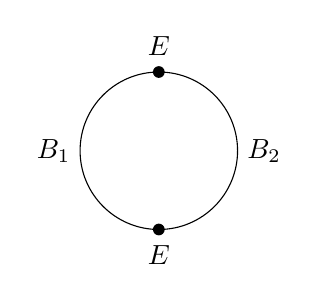
\begin{tikzpicture}[%every label/.style={green}
]
\node[fill=black, circle, label=below:$E$, inner sep=1.5pt](S) at (0,0) {};
\node[fill=black, circle, label=above:$E$, inner sep=1.5pt](N) at (0,2) {};
\draw (S) arc  (-90:90:1);
\draw (N) arc  (90:270:1);
\node[left] at (-1,1) {$B_1$};
\node[right] at (1,1) {$B_2$};
\end{tikzpicture}
\caption{Combining two balls to get a full boundary.}\label{blah3}\end{figure}

\begin{figure}
\centering
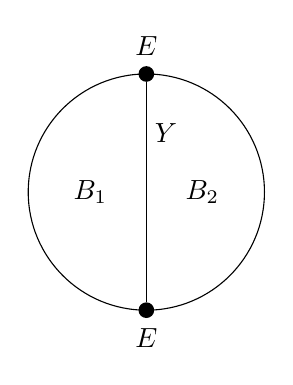
\begin{tikzpicture}[%every label/.style={green},
				x=1.5cm,y=1.5cm]
\node[fill=black, circle, label=below:$E$, inner sep=2pt](S) at (0,0) {};
\node[fill=black, circle, label=above:$E$, inner sep=2pt](N) at (0,2) {};
\draw (S) arc  (-90:90:1);
\draw (N) arc  (90:270:1);
\draw (N) -- (S);
\node[left] at (-1/4,1) {$B_1$};
\node[right] at (1/4,1) {$B_2$};
\node at (1/6,3/2)  {$Y$};
\end{tikzpicture}
\caption{From two balls to one ball.}\label{blah5}\end{figure}

\begin{figure}
\begin{equation*}
\mathfig{.23}{ncat/zz2}
\end{equation*}
\caption{A small part of $\cell(W)$.}
\label{partofJfig}
\end{figure}

\begin{figure}
$$\mathfig{.4}{deligne/manifolds}$$
\caption{An $n$-dimensional surgery cylinder.}\label{delfig2}
\end{figure}


%% For Tables, put caption above table
%%
%% Table caption should start with a capital letter, continue with lower case
%% and not have a period at the end
%% Using @{\vrule height ?? depth ?? width0pt} in the tabular preamble will
%% keep that much space between every line in the table.

%% \begin{table}
%% \caption{Repeat length of longer allele by age of onset class}
%% \begin{tabular}{@{\vrule height 10.5pt depth4pt  width0pt}lrcccc}
%% table text
%% \end{tabular}
%% \end{table}

%% For two column figures and tables, use the following:

%% \begin{figure*}
%% \caption{Almost Sharp Front}\label{afoto}
%% \end{figure*}

%% \begin{table*}
%% \caption{Repeat length of longer allele by age of onset class}
%% \begin{tabular}{ccc}
%% table text
%% \end{tabular}
%% \end{table*}

\end{document}

